%This work is licensed under the Creative Commons License Attribution 4.0 International (CC-BY 4.0) 
%https://creativecommons.org/licenses/by/4.0/legalcode 
\documentclass[rgb]{standalone}
\usepackage{tkz-euclide}
\begin{document}
	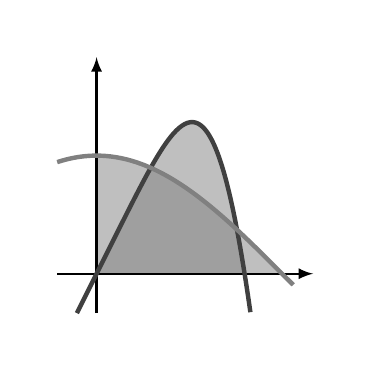
\begin{tikzpicture}[scale=0.5, font=\Large]
		\draw[draw=none] (-1.75,-1.75) -- (-1.75,6.25) -- (6.25,6.25) -- (6.25,-1.75) -- cycle;
		\draw[draw=none,fill,gray,fill opacity=0.5,domain={0}:{sqrt(pi/2)}, smooth, samples=1500, variable=\x] (0,0) -- plot (3*\x, {6*\x*cos(\x*\x*180/pi)}) -- ({2*sqrt(pi/2)},0);
		\draw[draw=none,fill,gray,fill opacity=0.5,domain={0}:{pi/2}, smooth, samples=300, variable=\x] (0,0) -- plot (3*\x, {3*cos(\x*180/pi)}) -- ({pi},0);
		\draw[thick, -latex] (-1,0) -- (5.5,0);
		\draw[thick, -latex] (0,-1) -- (0,5.5);
		\draw[ultra thick,domain={-0.16673}:{1.30346}, smooth, samples=300, variable=\x,darkgray] plot (3*\x, {6*\x*cos(\x*\x*180/pi)});
		\draw[ultra thick,domain={-1/3}:{5/3}, smooth, samples=300, variable=\x,gray] plot (3*\x, {3*cos(\x*180/pi)});
	\end{tikzpicture}
\end{document}